\section{Évaluation des livrables}
       \subsection{Dossier d'expression des besoins}
              \subsubsection{Étude de l'existant}
Nous avons mis en valeur l'existant organisationnel, informatique, les processus stratégiques (pour la facturation, l'approvisionnement, la demande matériel, la maintenance et la planification).Nous avons aussi mentionné les dysfonctionnements.

              \subsubsection{Benchmarking}
Nous avons procédé à un benchmarking non seulement au niveau des entreprises du même secteur d'activité (entreprises leaders du marché dans la construction), mais aussi au niveau des outils utilisés (ERP utilisés au sein des entreprises de BTP).

              \subsubsection{Thèmes de progrès}
Nous avons distingué les thèmes de progrès stratégique, organisationnel, fonctionnel, technologique.

       La principale difficulté était liée au benchmarking, surtout celui concurrentiel, les grandes entreprises fournissent peu d'informations (car celles ci sont liées à leur stratégie) et les petites et moyennes entreprises en fournissent beaucoup trop, mais surtout des informations non pertinentes, on a eu l'impression de ne pas avoir d'informations pertinentes sur leurs bests practices après avoir benchmarké.

       \subsection{Dossier de scenarii}
Nous avons proposé une architecture applicative avec un découpage en pacquage, l'architecture logicielle et technique correspondaient également à nos prévisions. Le plus dans cette phase, est le choix de la mise en place d'un intranet et du déploiement de nos applications sur une plateforme web.

       La principale difficulté durant cette phase a été de mettre à jour les modèles. Certains modèles existants étaient complexes, il fallait bien les comprendre et y rajouter nos thèmes de progrès sans les altérer pour autant.

       \subsection{Dossier de choix}
On a recensé les sources de dépense puis on a effectué l'évaluation des coûts (investissement, maintenance, formation), le plan de mise en œuvre (les délais), les gains et retours sur investissement, ainsi que l'évaluation des risques.

        L'évaluation des coûts et des gains est très difficile à faire, les valeurs proposés se basent uniquement sur nos jeunes expériences et quelques recherches. Il en est de même pour l'évaluation des risques, après les avoir recensés, définir les coûts qui y sont liés est complexe.

       \subsection{Dossier de bilan}
En plus de la description de l'évolution des livrables, du bilan des charges et de la synthèse des difficultés rencontrées, on a rajouté également les bilans personnels et un annexe (contenant le diagramme de gannt final et les deux derniers tableau de bord d'avancement)


\section{Bilan des charges}
Il est important d'évaluer les charges des ressources (les 7 membres de l'équipe). Ainsi, grâce à ce bilan, nous pouvons voir les ressources qui ont eu plus de travail que d'autres et comparer celles-ci entre elles. Le bilan des charges fournit pas MS Project étant trop détaillé, nous l'avons résumé dans ce tableau, mais ce bilan détaillé est proposé en annexe.
\\~\\
\begin{tabular}{c c c c c c c c}
    \multirow{3}{*}{~} & Organisation & \multicolumn{3}{c}{Expression des besoins} & Scénarios & Évaluation & \multirow{2}{*}{Total} \\
    & du projet & & & & & &\\
    & S1 & S2 & S3 & S4 & S5 & S8 & \\
    \hline
    Naby & 13.8 & 2.3 & 4.3 & 9.3 & 6.3 & 7.3 & 43.3 \\
    Etienne & 9 & 2 & 2 & 3 & 4 & 6 & 26.0 \\
    Johann & 2.25 & 3.25 & 3.25 & 3.25 & 4.25 & 4.25 & 20.5 \\
    Baptiste & 2.5 & 2 & 4 & 4 & 3 & 4 & 19.5 \\
    Chafik & 3 & 4 & 2 & 6.25 & 2 & 4 & 21.25 \\
    Thanh & 2 & 4 & 2 & 4.25 & 4 & 4 & 20.25 \\
    Adrien & 2.5 & 4 & 2 & 3.75 & 4 & 4 & 20.25 \\
    \hline
    Equipe & 4.6 & 0.6 & 0.6 & 0.6 & 0.6 & 6.6 & $7\times13.6$ = 95.2 \\
    \hline
    Total & \multicolumn{6}{c}{~} & 266.25
\end{tabular}
\\~\\
Par ailleurs, une ressource a été consacrée à l'ensemble de l'équipe, cette ressource s'appelant « Equipe ». Elle permet de comptabiliser le temps consacré aux réunions (de chantier, de résolution de problèmes, de coordination..), qui monopolisent toute l'équipe et représente tout de même un temps conséquent sur le projet.

Par rapport au contenu, nous sommes satisfait, nos livrables non pas vraiment évolués en termes de contenu, nous avions eu durant la phase d'initialisation, une bonne compréhension du produit attendu. 

Les écarts sont surtout dû à l'identification des tâches et à l'estimation du temps de travail, j'avais une vue macro au mieux de l'ensemble des tâches et ma jeune expérience ne m'a pas permis d'effectuer un chiffrage précis du temps de travail, mais il faut avouer que cette tâche est assez complexe.

\section{Synthèse des difficultés rencontrées}

          En tant que chef de projet, je me suis rendu compte de la difficulté qu'était de gérer un tel projet en terme d'organisation, de cohérence des livrables. Au delà d'affecter des tâches aux collaborateurs et de superviser leur  travail, il faut cadrer le champ de travail, guider les recherches, servir de conseiller car on a une vue générale du projet. La taille du projet m'a réellement permis de m'imprégner de ce poste et d'en découvrir les difficultés au quotidien. 

         Certaines difficultés ont déjà été évoquées expliquant l'origine des écarts du plan de charges notamment l'identification et l'estimation des tâches constituant le projet en général. Il était difficile pour ma part de définir une tâche précise, de l'estimer car nous n'avons pas eu assez d'informations. Bien
entendu, je comprenais que c'était une estimation et non un temps de travail exact. 

          De plus, une autre difficulté était l'attribution des tâches aux membres de l'équipe. Sachant que chacun avait un rôle il fallait leur attribuer des tâches liées à leur poste tout en essayant d'équilibrer la charge de travail sur l'ensemble du projet. Ce qui a fait que selon les séances, certaines ressources étaient plus sollicitées que d'autres, mais ce fût une réelle gymnastique intellectuelle. Et il fallait y parvenir, car plus il travaillerait sur des tâches similaires, plus leur expertise en serait meilleure.

         L'une des autres difficultés importantes était d'assurer la communication en interne, durant certaines séances une partie importante de l'équipe était mobilisé afin de vérifier la cohérence de nos idées. Suite aux réunions avec le client, le responsable communication effectuait un petit résumé à l'équipe pour informer des éventuelles changements.

        La dernière difficulté à signalé me concerne plus particulièrement, ma crainte des incohérences et le souci de présenter des livrables de qualité m'a amené à trop cadré le champ du projet, j'ai certainement laissé place à peu d'imaginations par moment à mes collaborateurs car je les allouais souvent des tâches assez précises et je savais ce que j'attendais comme résultat. Ce qui a d'ailleurs fait que j'ai pas mal participé à la production quand je n'étais pas entièrement satisfait de leurs livrables intermédiaires. Au fur et à mesure, ce projet m'a appris à prendre plus de recul sur le travail des autres.

      Malgré les difficultés évoquées, ce projet m'a apporté un meilleur regard sur le poste de chef de projet, et je suis satisfait du travail effectué par mes collaborateurs, le projet a été mené à bout dans les délais et dans de bonnes conditions de travail.


\section{Bilans Personnels}

    \subsection{DIAKITE Naby Daouda (Chef de projet)}

        Ce projet s’est avéré intéressant sous plusieurs aspects. C’est le premier projet que j’effectue en tant que chef de projet, en dehors de CIAI, qui ne présente pas vraiment d’intérêt dans la gestion de projet.

        J’ai ici pu approcher la perspective d’un véritable chef de projet, en me concentrant sur la gestion du projet, de l’équipe. 

        La taille conséquente du projet m’a permis d’approfondir certains points. C’est une première expérience extrêmement intéressante, qui m’a conforté dans l’idée que je m’étais fait de la conduite de projet, et qui n’a que renforcé mon attraction pour cette fonction.

        La principale difficulté dans un projet « scolaire » censé simuler une situation réelle est l’absence de réel poids hiérarchique. En effet, dans la vie réelle un employé dépend directement de son chef,  alors que dans notre situation il ne s’agit que d’étudiants qui jouent un rôle. Il n’est donc pas toujours évident d’avoir une autorité légitime sur le reste du groupe.

        J’ai cependant apprécié le fait que chacun joue le jeu, et s’attache à réaliser ses tâches.

        Les membres de l'équipe se sont bien intégrés et l'environnement de travail était agréable.

    \subsection{BRODU Etienne (Responsable qualité)}

        Si j'ai choisi ce rôle de responsable qualité pendant ce projet, c'est avant tout pour avoir une idée concrète de la gestion de la documentation sur un projet suffisamment conséquent afin d'avoir les repères pour améliorer cette gestion, et les communications au sein de l'équipe.\\
        C'est donc dans le but d'améliorer la productivité que j'ai choisi ce rôle, avec comme idée de base de se concentrer plus sur le fond que sur la forme.
        Bien que cet objectif ne soit qu'à moitié rempli, je suis content du résultat.\\
        \\
        Il est en effet très dur de faire accepter un outils commun à une équipe dont chacun des membres à déjà ses propres outils hétérogène.
        Cependant la plupart des membres de l'équipe ont joué le jeux et on réussi à maitriser plusieurs outils qu'ils ne connaissaient pas avant.

    \subsection{CHAZELLE JOHANN (Responsable communication)}

        \subsubsection{Contexte}
        Nous avons, pour la première fois, pris part à un projet de 3 mois environ. Une expérience intéressante dont l’objectif était de présenter une ou plusieurs solutions s’attachant à moderniser le système d’information de la gestion du matériel d’une entreprise de travaux public, GSTP.
        Spécification des besoins
        Lors de la première phase du projet, une étude approfondie a été menée sur l’existant de GSTP et sur les moyens utilisés par la concurrence. Des axes d’améliorations ont ainsi pu être dégagés, première étape dans la spécification d’une solution propre à GSTP.
        Étant intéressé par le monde de l’avant-vente, la compréhension du métier m’attire particulièrement. Cependant, dans le cadre de notre étude, des recherches limitées au Web (notre temps restant réduit) m’ont semblé peu fructueuses. Nous avons pu obtenir quelques informations, mais pas nous plonger véritablement dans les aspects métiers relevant d’une entreprise réelle du BTP.

        \subsubsection{Solution spécifique}
        Cinq membres de l’équipe se sont lancés sur un projet spécifique, ainsi notre étude c’est limitée à celle d’une solution spécifique. A partir des axes d’amélioration définis dans la partie précédente nous avons pu proposer notre solution.
        Malgré des attentes ciblées peut-être quelque fois, plus par les professeurs que par le client (en termes de modélisation notamment), cette partie nous a offert une liberté importante en ce qui concerne l’imagination d’une solution complète.

        \subsubsection{Un travail d’équipe}
        Ce projet, tout comme le projet d’ingénierie nous a permis d’appliquer un mode d’organisation jusqu'ici difficile à mettre en place dans nos projets scolaires (souvent par manque de temps). Ainsi, les rôles attribués à chacun, avec des responsabilités bien précises, s’approchent bien plus de ceux que nous retrouvons dans le contexte réelle d’une entreprise ce qui est particulièrement intéressant et formateur.

        \subsubsection{Conclusion}
        Ce projet nous est présenté sous une forme intéressante nous permettant de travailler sur des tâches situées en amont de celles expérimentées dans les projets habituels. Cependant, le manque de temps sur certaines tâches (benchmarking), ou l’orientation par le corps enseignant vient parfois nous rappeler que ce projet reste un projet scolaire.


    \subsection{LECORNU Baptiste (Expert ERP/Modélisation)}
        Mon rôle durant le projet fut, au départ, expert ERP. Le problème, c’est qu’en milieu de projet nous avons décidés de faire un projet spécifique en dehors des cours. En accord avec le corps enseignant, nous avons donc décidés de ne pas faire le scénario ERP pour nous libérer des séances pour le projet spécifique. J’ai donc ‘’perdu’’ deux séances à me renseigner sur les ERPs, pour au final très peu utiliser ces informations. De ce fait, je n’ai pas l’impression d’avoir été très actif sur ce TP, bien que j’ai travaillé normalement les autres séances. 
        Mis à part ça, ce projet était riche pédagogiquement parlant. On a du toucher à un peu tous les cours de ERP et gestion de projet. Et le principe d’équipe est vraiment intéressant, on voyait bien ici l’intérêt du chef de projet et du responsable qualité.
        La charge de travail m’a semblait raisonnable, il m’a fallu travailler peu en dehors des séances.
        Le groupe H4212 reste pour moi un très bon groupe, auquel je suis attaché. Nous venons tous d’horizons différents et pourtant nous avons su former une équipe plutôt soudée où la communication règne.

    \subsection{BACHATENE Chafik (Expert métier achat)}

        Le projet PLD m'a semblé non sans intérêt de part sa nature à regrouper l'approche ERP et l'étude d'un système d'information et ses objectifs pédagogiques.
        Partir d'un cas concret se rapprochant de la réalité et traitant d'un sujet très répandu (le BTP) l'a rendu davantage intéressant. Par ailleurs, et bien que les différentes parties étaient bien structurées, il y avait très souvent un sentiment de frustration lorsqu'à l'issue d'une séance on ne produisait que de la documentation. Aussi la partie étude , ou plus exactement recherche sur internet,bien que nécessaire, nous donnait l'impression de toucher à des secteurs et des domaines très loin de l'informatique. 
        L'absence des aspects techniques nous a montré que l'élaboration d'un système d'information ne se réduisait pas au simple développement d'un logiciel. 
        L'ambiance de travail était très agréable, les rôles étaient bien répartis en fonction des profils. Le chef de projet a bien su motiver l'ensemble du groupe, en particulier dans la partie modélisation où nous étions un peu perdu et ne savions pas exactement ce qu'il nous été demandé. Il s'est investi et a expliqué très clairement ce que nous devions faire.
        Je trouve néanmoins dommage de ne pas avoir eu suffisamment de temps pour discuter et débattre des idées et solutions de chaque membre de l'équipe. la répartition des rôles réduit quelques peut le panel d'idées proposées. 

    \subsection{PHAN DUC Thanh (Expert métier maintenance)}

        Au début on a pensé que ce projet n'était pas intéressant, car il y a aucun code à produire. Au final on a compris qu'il était très utile car il nous a permis de pénétrer dans le monde du projet SI d'entreprise. On a pu découvrir les démarches d'un tel projet: étude préalable, benchmarking. Il nous a permis aussi de comprendre la définition des critères de comparaison, la pondération des ces critères et puis leurs applications.  En plus, on a a découvert non seulement les aspects fonctionnels mais aussi commerciaux d'un projet d'entreprise.\\

        Ce projet est donc un ajout important dans notre formation d'ingénieur car il nous a permis aussi de prendre conscience de nos défauts, de nos points forts de manière à pouvoir mieux appréhender certaines difficultés à l'avenir. 

    \subsection{BROCHOT Adrien (Expert métier gestion de matériels)}

        En tant que membre du groupe d'étude informatique, j'ai trouvé que ce projet nous a totalement immergé dans un cadre professionnel. Durant ce projet, nous avons effectué un travail d'étude et d'analyse dans un contexte réel. Il nous a fourni une mission réaliste qu'il nous a fallu remplir en travaillant tous ensemble au sein d'un groupe de travail organisé.\\
        \\
        Ce projet a poussé bien plus loin les rôles assignés aux différents membres de l'hexanôme et nous a contraint à nous organiser et à effectuer des tâches spécifiques à chaque poste. Je suis personnellement satisfait de cette expérience qui m'a permis de découvrir le travail en groupe et l'importance de chaque acteur du groupe.\\
        \\
        La principale difficulté au cours de ce projet a été pour moi la production de livrables cohérents et homogènes par rapport au travail des autres membres du groupe d'étude.\\
        \\
        L'équipe du groupe d'étude a rédigé de nombreux livrables au cours de ce projet et garantir la cohérence de notre production n'était pas toujours facile : il fallait parfois modifier d'anciens dossiers et intégrer ces modification logiquement dans la suite du projet. Notre chef de projet, dans le but de limiter les incohérences, a organisé de nombreuses réunions afin de mettre en commun notre travail de manière plus simple que par consultation du répertoire partagé. Nous avons donc pu largement améliorer la cohérence globale du projet grâce à ces mises en commun régulières.\\
        \\
        La charge de travail ne m'a pas paru trop importante compte tenu de l'ampleur du projet. La répartition sur chaque séance était cependant assez variable et nous a parfois contraint à travailler beaucoup entre deux séances alors que nous n'avons globalement pas énormément travaillé hors séance.\\
        \\
        L'ambiance de travail tout au long du projet était très bonne et nous avons tous pu travailler en commun. Je pense que notre groupe a réussi à travailler efficacement en équipe sans qu'il y ait eu de tensions particulières entre les différents membres.\\
        \\
        Pour conclure, je retire de ce projet une expérience très intéressante de travail en groupe organisé et une meilleure vision d'ensemble d'un tel projet.

\section{Annexes}

    \subsection{Diagramme de GANTT Final (MS Project)}
        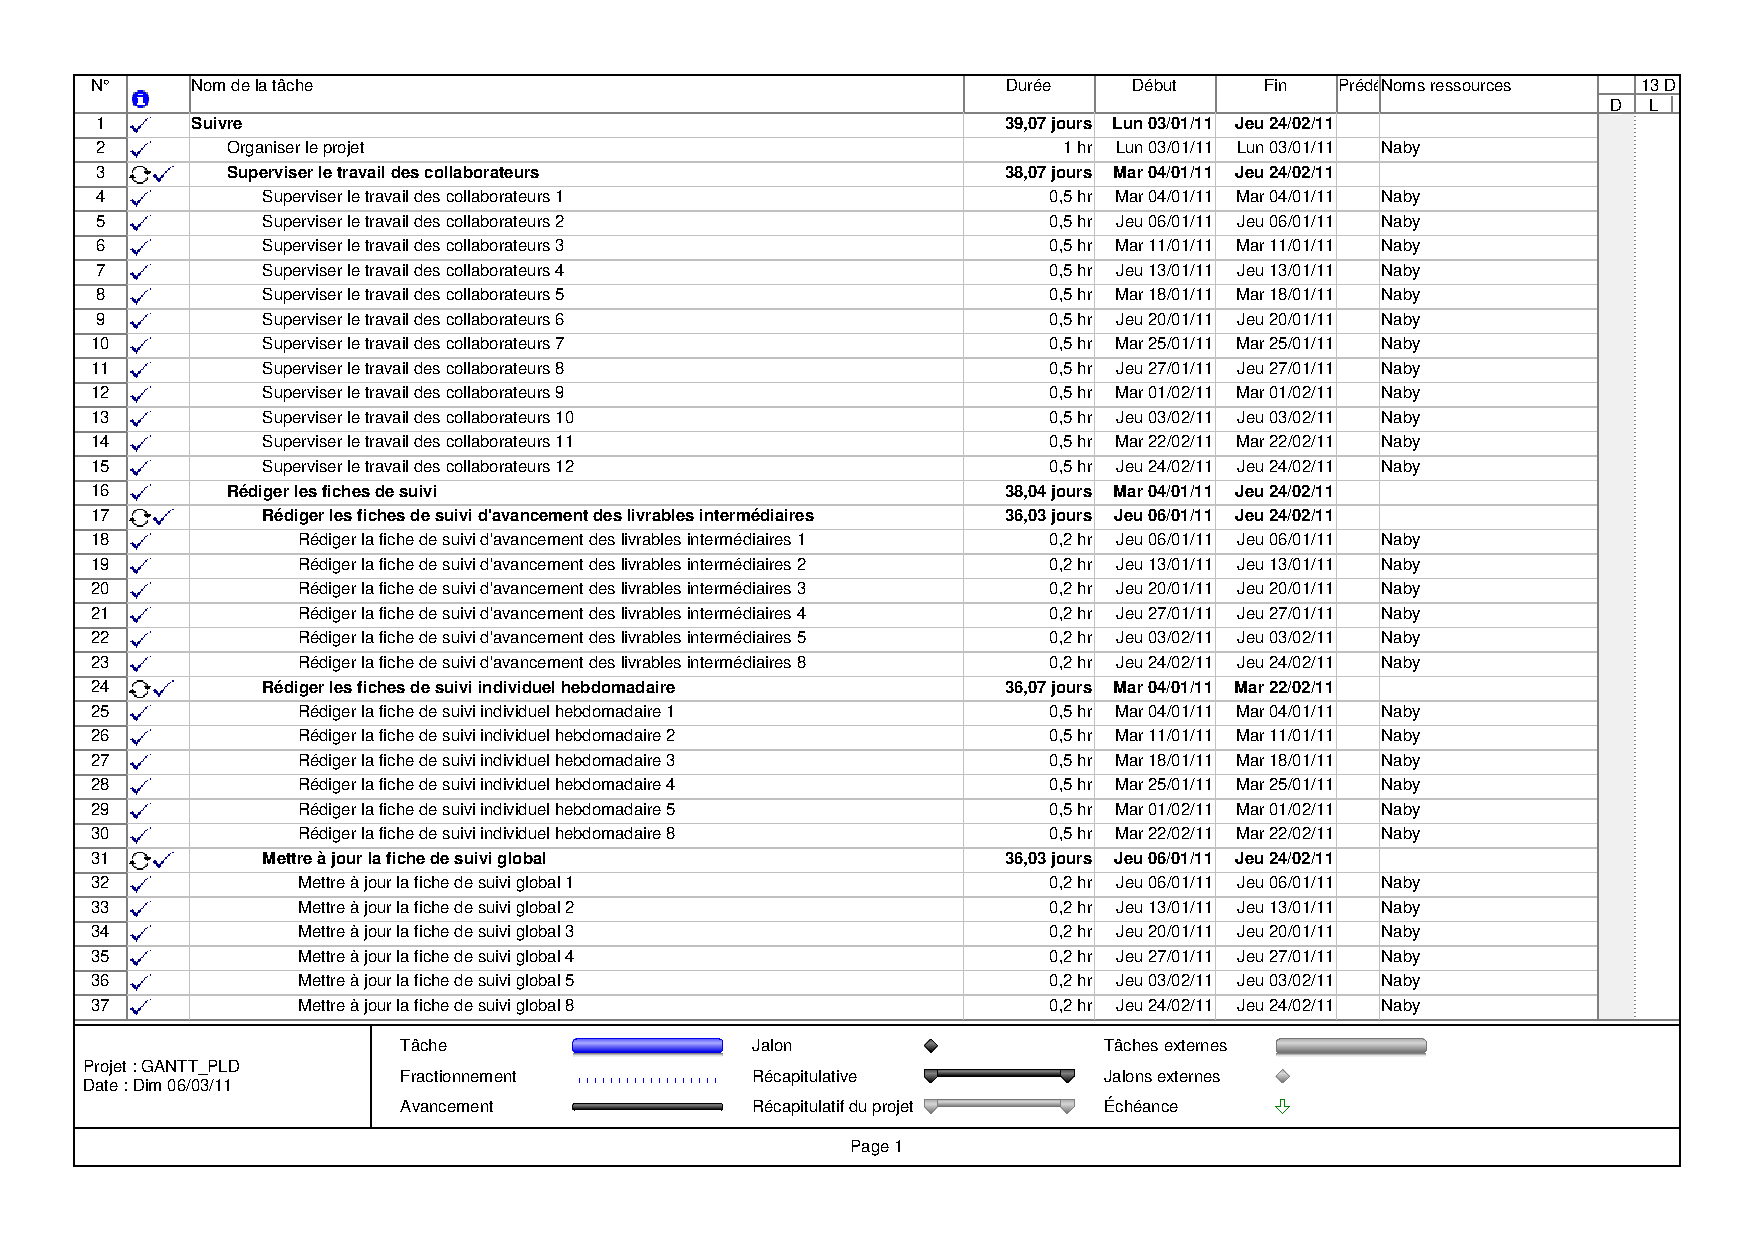
\includepdf[landscape = true, pages=1-6]{img/gantt.pdf}

    \subsection{Tableau de bord avancement}
        \begin{tabular}{l c}
            \textbf{Indicateur} & \textbf{Bilan après la phase : P4} \\
            \hline
            Charge initiale du projet & 228.05 h \\
            Charge globale du projet à l’instant t & 266, 25 h \\
            Réalisé prévu à l’instant t & 266, 25 h \\
            Réalisé effectif à l’instant t & 266, 25 h \\
            Avancement prévu & 100 \% \\
            Avancement réel & 100 \% \\
            Retard & 0\% \\
        \end{tabular}





